\documentclass[12pt, varwidth, border={5mm 5mm 5mm 5mm}]{standalone}
\usepackage{tikz}
\usepackage{amsmath}
% Underlining package
\usepackage{ulem}
\usetikzlibrary{calc}
% \usepackage[a4paper, portrait, margin=1cm]{geometry}

\begin{document}
\section*{ }
    \begin{minipage}{0.55\textwidth}
  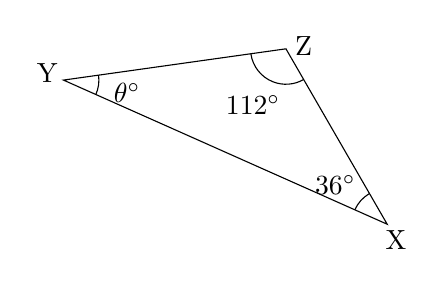
\begin{tikzpicture}[scale=1.5, baseline=(current bounding box.south)]
    \pgfmathsetmacro{\angleA}{32}
    \pgfmathsetmacro{\angleB}{36}
    \pgfmathsetmacro{\angleC}{112}
    \pgfmathsetmacro{\sideC}{3}
    \pgfmathsetmacro{\rotationAngle}{336}

    \begin{scope}[rotate=\rotationAngle]
      \coordinate (A) at (0,0);
      \coordinate (B) at (\sideC,0);
      \coordinate (C) at (intersection cs: first line={(A)--($(A)+(\angleA:4cm)$)}, second line={(B)--($(B)+(180-\angleB:4cm)$)});
      \draw (A) -- (B) -- (C) -- cycle;
      
      % Mark angles with arcs
      \draw ($(A)!0.3cm!(B)$) arc [start angle=0, end angle=\angleA, radius=0.3cm];
      \draw ($(B)!0.3cm!(C)$) arc [start angle=180-\angleB, end angle=180, radius=0.3cm];
      \draw ($(C)!0.3cm!(A)$) arc [start angle=180+\angleA, end angle=360-\angleB, radius=0.3cm];
      
      % Label angles
      \node at ($(A)!-0.15cm!(B)$) {Y};
      \node at ($(B)!-0.15cm!(C)$) {X};
      \node at ($(C)!-0.15cm!(A)$) {Z};
      
      % Mark angles in degrees
      \coordinate (midBC) at ($(B)!0.5!(C)$);
      \node at ($(A)!0.55cm!(midBC)$) {$\theta ^\circ$};
  
      \coordinate (midAC) at ($(A)!0.5!(C)$);
      \node at ($(B)!0.55cm!(midAC)$) {36$^\circ$};
  
      \coordinate (midAB) at ($(A)!0.5!(B)$);
      \node at ($(C)!0.55cm!(midAB)$) {112$^\circ$};
    
    \end{scope}
  \end{tikzpicture}
\end{minipage}%
\hfill
\begin{minipage}{0.4\textwidth}
  \begin{align*}
    \angle \text{Y} &= 180^\circ - (\angle \text{X} + \angle \text{Z}) \\
    &= 180^\circ - (\dotuline{~~~~~~~}^\circ + \dotuline{~~~~~~~}^\circ) \\
    &= 180^\circ - \dotuline{~~~~~~~}^\circ \\
    &= \dotuline{~~~~~~~}^\circ
  \end{align*}
\end{minipage}
\end{document}
